\section{Thiết kế hệ thống và Lý giải kiến trúc}
\label{sec:design}

\noindent \textbf{Kiến trúc tổng thể và Luồng điều khiển (\texttt{R1}).} SQLGuard tách rạch ròi tầng \textit{suy luận đề xuất} (Planner) khỏi tầng \textit{kiểm soát thực thi} (Gate, Tool, DB Authorizer), minh họa ở Hình~\ref{fig:architecture}. Khi nhận câu hỏi kèm phiên đăng nhập đã xác thực (\texttt{SecurityContext}), hệ thống nạp schema đã lọc theo role và ngữ nghĩa nghiệp vụ để Planner sinh câu lệnh SQL. Câu lệnh phải vượt qua \texttt{PolicySQLGate} (sinh lại \texttt{normalized\_sql} từ AST) $\rightarrow$ \texttt{SecureSqlTool} (kiểm lại và giới hạn dòng) $\rightarrow$ \texttt{SQLiteAuthorizer} (chốt chặn tầng DB) trước khi trả kết quả sạch về cho người dùng. Vòng điều phối \texttt{AgentController} khóa ngân sách \texttt{ExecutionBudget}: tối đa 6 lượt gọi Planner, 8 lượt gọi Tool, tối đa 3 lần thử SQL, timeout 3s/truy vấn và 60s/run.

\begin{figure}[H]
    \centering
    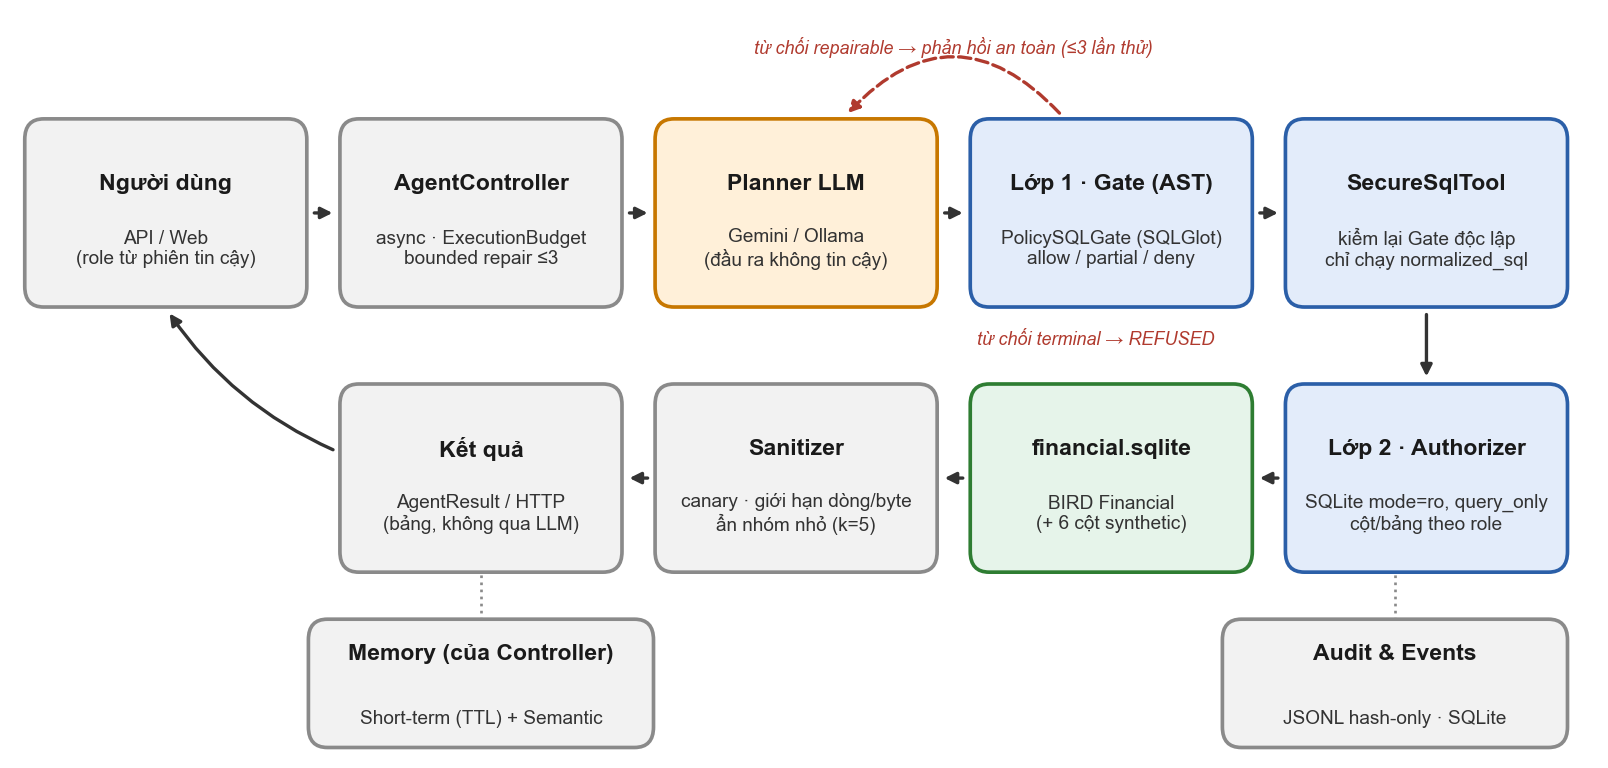
\includegraphics[width=0.72\linewidth]{figures/architecture.png}
    \caption{Kiến trúc tổng thể và luồng kiểm soát nhiều lớp của SQLGuard}
    \label{fig:architecture}
\end{figure}

\noindent \textbf{Công cụ MCP và Mức phân quyền (\texttt{R2}).} Thay vì giữ 3 tool như đề xuất D1, nhóm chủ động hợp nhất \texttt{sanitize\_data} vào bên trong \texttt{SecureSqlTool} để bảo đảm tính tối giản (\textit{simplicity argued}): LLM không thể gọi truy vấn mà bỏ qua bước làm sạch. Mọi tham số \texttt{role} đều được lấy từ phiên backend, không xuất hiện trong schema tham số của tool (Bảng~\ref{tab:mcp-tools}).

\begin{table}[htbp]
\centering
\caption{Phân loại mức quyền công cụ trong SQLGuard (\texttt{R2})}
\label{tab:mcp-tools}
\footnotesize
\renewcommand{\arraystretch}{1.15}
\begin{tabular}{|l|l|p{0.28\linewidth}|p{0.34\linewidth}|}
\hline
\rowcolor{tableheader}
\textbf{Công cụ / Thành phần} & \textbf{Mức quyền (\texttt{R2})} & \textbf{Chức năng} & \textbf{Cơ chế kiểm soát} \\ \hline
\texttt{get\_schema} (MCP) & \texttt{read-only} & Trả bảng/cột hợp lệ của role & Lọc sẵn theo \texttt{SecurityContext}; không nhận tham số \texttt{role} \\ \hline
\texttt{query(sql)} (MCP) & \texttt{read-only} & Chạy 1 câu \texttt{SELECT} chỉ đọc & AST Gate $\rightarrow$ tái kiểm tra $\rightarrow$ \texttt{normalized\_sql} $\rightarrow$ Authorizer $\rightarrow$ Sanitizer \\ \hline
\texttt{AttackLab} (Admin UI) & \texttt{reversible-write} & Tiêm/khôi phục payload lab & Tách khỏi Agent; chỉ \texttt{admin}; bản sao DB + \texttt{expected\_revision} + Restore \\ \hline
\textit{Irreversible write} & \texttt{none (0 tools)} & Không cung cấp & Chặn tuyệt đối DDL/DML ở Gate, chế độ \texttt{mode=ro} và Authorizer \\ \hline
\end{tabular}
\end{table}

\noindent \textbf{Thiết kế Bộ nhớ (\texttt{R3}) và Ba trục nâng cao (\texttt{R4}).}
\begin{itemize}
    \item \textbf{Memory (\texttt{R3}):} (1) \textit{Short-term Memory} (\texttt{InMemoryMemory}, TTL 1 giờ, phân vùng theo \texttt{run\_id}): \textit{Write policy} chỉ do Controller ghi mã trạng thái, mã lỗi và số retry (không lưu dữ liệu DB thô); \textit{Retrieval policy} chỉ nạp ngữ cảnh cùng \texttt{run\_id} cho bước \texttt{repair\_plan}. (2) \textit{Semantic Memory} (\texttt{SemanticMemory}, phiên bản theo policy): \textit{Write policy} là chỉ đọc tại runtime (chỉ cập nhật qua mã nguồn đã duyệt, cấm Agent tự ghi nhằm chống \textit{memory poisoning}); \textit{Retrieval policy} lọc định nghĩa nghiệp vụ theo đúng bảng/cột role được phép và bọc nhãn không tin cậy.
    \item \textbf{Ba trục nâng cao (\texttt{R4}):} (1) \textit{AST Column Guardrails \& Rewriting} (\texttt{PolicySQLGate} + \textit{Partial Answer} + ẩn nhóm $k<5$); (2) \textit{Bounded Reflection} phân tách \texttt{repairable} vs \texttt{terminal}; và (3) \textit{Multi-layer Sandboxed Verification} (\texttt{SecureSqlTool} + \texttt{SQLiteAuthorizer} + canary/sanitizer).
\end{itemize}
